\part{Software Requirements Specification}

\section{Introduzione}
\subsection{Scopo del documento}
Questo documento specifica i requisiti di [Nome], il backend di un
applicativo per Personal Trainer. Il documento descrive gli attori del
sistema, i concetti del dominio e i casi d'uso.

\subsection{Descrizione del progetto}
L'applicativo digitalizza la gestione degli atleti di un Personal
Trainer. Il PT crea le schede di allenamento e le assegna ai propri
atleti. Il PT e i suoi atleti fissano inoltre gli appuntamenti di
allenamento in comune.

Il sistema ha due attori:
\begin{itemize}
  \item \textbf{PT}: offre il servizio. Registra i propri atleti. Crea
    le schede e le assegna agli atleti. Gestisce le richieste di
    appuntamento che riceve dagli atleti.
  \item \textbf{Atleta}: riceve il servizio dal PT. Consulta le schede
    che il PT gli ha assegnato. Richiede gli appuntamenti con
    il PT.
\end{itemize}

% \subsubsection{Struttura di una scheda}
% Una scheda ha tre livelli:
% \begin{itemize}
%   \item la scheda contiene uno o più blocchi mensili;
%   \item ogni blocco mensile contiene le sessioni di allenamento di
%     quattro settimane;
%   \item ogni sessione di allenamento contiene gli esercizi da eseguire.
% \end{itemize}
% La scheda definisce quali esercizi l'atleta esegue e come li esegue,
% cioè le serie, le ripetizioni, il tempo di recupero e la variante di
% esecuzione. La scheda non definisce i carichi.
%
% \subsubsection{Riuso di una scheda}
% Il PT può assegnare la stessa scheda a più atleti. Il PT inserisce i
% carichi al momento dell'assegnazione, perché il carico è specifico
% dell'atleta. Il PT indica anche la data di inizio. Il sistema calcola
% la data di fine dal numero di blocchi mensili della scheda.
%
% Il PT può modificare i valori prescritti a un singolo atleta con la
% personalizzazione. La personalizzazione non modifica la scheda e non ha
% effetto sugli altri atleti che seguono la stessa scheda.

\subsection{Definizioni e abbreviazioni}
\begin{description}
  \item[PT] Personal Trainer. È l'utente che offre il servizio e che
    usa l'applicativo per gestire i propri atleti.
  \item[Atleta] L'utente finale che riceve il servizio dal PT.
  \item[Scheda] Il piano di allenamento. Raggruppa uno o più blocchi
    mensili. Il PT può assegnare la stessa scheda a più atleti.
  \item[Blocco mensile] Il mese di allenamento di una scheda. Dura
    quattro settimane e contiene le sessioni di allenamento di quel
    mese.
  \item[Sessione di allenamento] L'insieme di esercizi che l'atleta
    esegue in un giorno di allenamento.
  \item[Esercizio] Il singolo movimento che l'atleta esegue in una
    sessione di allenamento. È descritto dal nome, dal gruppo
    muscolare, dalle serie, dalle ripetizioni, dal tempo di recupero e
    dalla variante di esecuzione.
  \item[Carico] Il peso che l'atleta solleva in un esercizio. Il PT lo
    inserisce per ciascun esercizio di ciascuna sessione, al momento
    dell'assegnazione.
  \item[Assegnazione] Il legame tra una scheda e un atleta. Contiene la
    data di inizio, la data di fine e i carichi di quell'atleta.
  \item[Bozza] Lo stato di un'assegnazione che il PT non ha ancora
    confermato. L'atleta non vede le assegnazioni in bozza.
  \item[Personalizzazione] La modifica dei valori di un esercizio
    limitata a una singola assegnazione.
  \item[Richiesta di appuntamento] La richiesta con cui l'Atleta chiede
    al PT un allenamento in comune. Contiene la data, l'ora e la
    motivazione. Il PT la conferma o la rifiuta.
  \item[Appuntamento] L'allenamento in comune tra il PT e l'Atleta, in
    una data e a un'ora stabilite. Nasce da una richiesta di
    appuntamento confermata.
\end{description}

\newpage
\section{Progettazione}
\subsection{Diagramma dei casi d'uso}
La figura \ref{fig:diagrammacasiduso} mostra i casi d'uso del sistema e
gli attori che li eseguono.
% \begin{figure}[H]
%   \centering
%   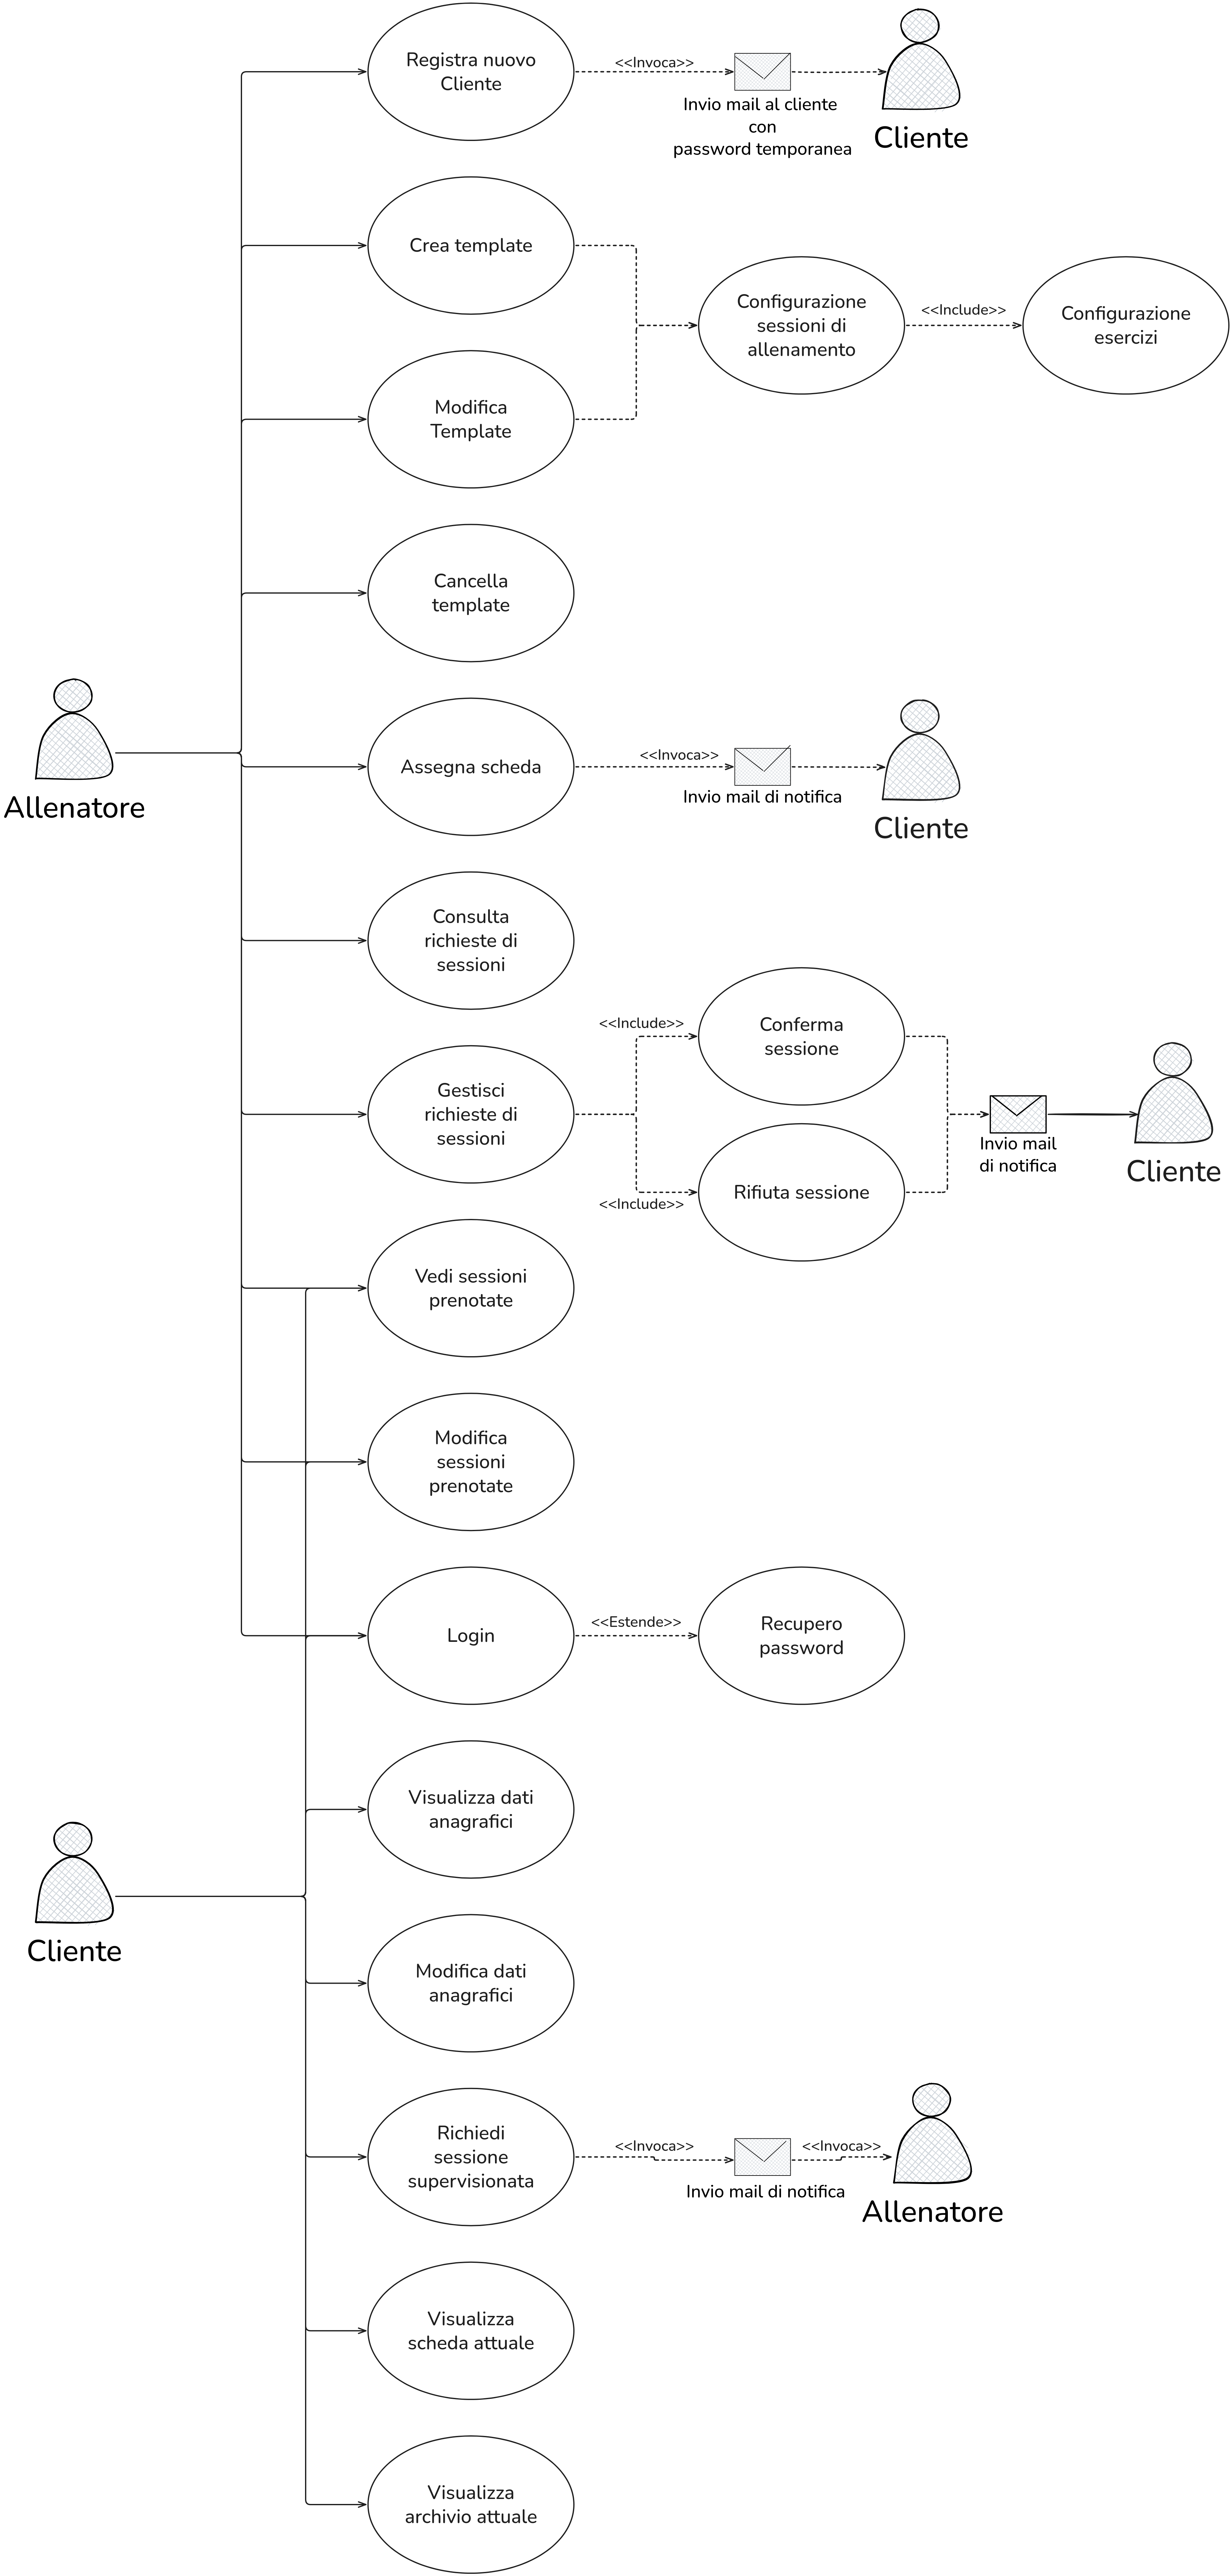
\includegraphics[width=0.5\textwidth]{diagrams/useCaseDiagram.png}
%   \caption{Diagramma dei casi d'uso}
%   \label{fig:diagrammacasiduso}
% \end{figure}

Il diagramma raggruppa i casi d'uso per attore primario. Il caso d'uso
U-01 (Login) è comune ai due attori. I casi d'uso PT-07 e A-05 hanno lo
stesso scopo, ma mostrano a ciascun attore i soli appuntamenti che lo
riguardano.

Le sezioni seguenti descrivono ciascun caso d'uso con un template. Il
codice del caso d'uso indica l'attore primario: U per i casi d'uso
comuni, PT per il Personal Trainer, A per l'Atleta.

\subsection{Template dei casi d'uso comuni}
\subsubsection{U-01: Login}
\subfile{../diagrams/useCaseTemplates/comuni/src/U-01-login}

\subsubsection{U-02: Recupero Password}
\subfile{../diagrams/useCaseTemplates/comuni/src/U-02-recuperoPassword}

\subsection{Template dei casi d'uso del PT}
\subsubsection{PT-01: Registrazione PT}
\subfile{../diagrams/useCaseTemplates/pt/src/PT-01-registrazionePT}

\subsubsection{PT-02: Registrazione nuovo Atleta}
\subfile{../diagrams/useCaseTemplates/pt/src/PT-02-registrazioneAtleta}

\subsubsection{PT-03: Creazione nuova Scheda}
\subfile{../diagrams/useCaseTemplates/pt/src/PT-03-creazioneScheda}

\subsubsection{PT-04: Configurazione Sessioni di Allenamento in una Scheda}
\subfile{../diagrams/useCaseTemplates/pt/src/PT-04-configurazioneSessioni}

\subsubsection{PT-05: Assegnazione Scheda ad un Atleta}
\subfile{../diagrams/useCaseTemplates/pt/src/PT-05-assegnazioneScheda}

\subsubsection{PT-06: Gestione Richiesta di Appuntamento}
\subfile{../diagrams/useCaseTemplates/pt/src/PT-06-gestioneRichiestaAppuntamento}

\subsubsection{PT-07: Visualizzazione Appuntamenti}
\subfile{../diagrams/useCaseTemplates/pt/src/PT-07-visualizzazioneAppuntamenti}

\subsubsection{PT-08: Visualizzazione Atleti}
\subfile{../diagrams/useCaseTemplates/pt/src/PT-08-visualizzazioneAtleti}

\subsubsection{PT-09: Personalizzazione di una Scheda Assegnata}
\subfile{../diagrams/useCaseTemplates/pt/src/PT-09-personalizzazioneScheda}

\subsubsection{PT-10: Modifica Scheda}
\subfile{../diagrams/useCaseTemplates/pt/src/PT-10-modificaScheda}

\subsubsection{PT-11: Cancellazione Scheda}
\subfile{../diagrams/useCaseTemplates/pt/src/PT-11-cancellazioneScheda}

\subsection{Template dei casi d'uso dell'Atleta}
\subsubsection{A-01: Completamento Profilo}
\subfile{../diagrams/useCaseTemplates/atleta/src/A-01-completamentoProfilo}

\subsubsection{A-02: Richiesta Appuntamento}
\subfile{../diagrams/useCaseTemplates/atleta/src/A-02-richiestaAppuntamento}

\subsubsection{A-03: Visualizzazione Schede Assegnate}
\subfile{../diagrams/useCaseTemplates/atleta/src/A-03-visualizzazioneSchede}

\subsubsection{A-04: Modifica Dati Anagrafici}
\subfile{../diagrams/useCaseTemplates/atleta/src/A-04-modificaDatiAnagrafici}

\subsubsection{A-05: Visualizzazione Appuntamenti}
\subfile{../diagrams/useCaseTemplates/atleta/src/A-05-visualizzazioneAppuntamenti}
